% The figure eight S^1 v S^1, with an open set U covering the left loop and a bit of the right.
% Source: book/tex/homology/long-exact.tex (§ Application: Mayer-Vietoris).
\documentclass[border=2mm]{standalone}
\usepackage{tikz}
\usetikzlibrary{calc}
\begin{document}
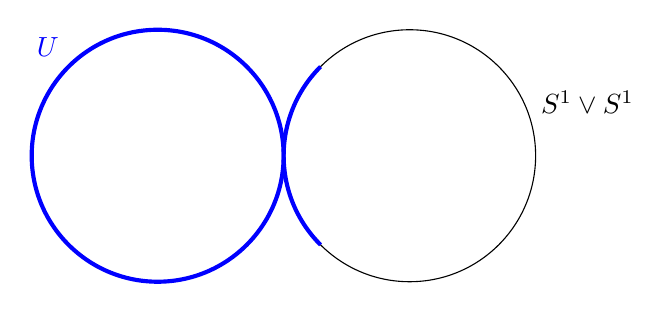
\begin{tikzpicture}[scale=1.6]
  \draw (0,0) circle (1);
  \draw[blue, line width=1.5pt] (-2,0) circle (1);
  \draw[blue, line width=1.5pt] (135:1) arc (135:225:1);
  \node[blue, above left] at ($(-2,0)+(135:1)$) {$U$};
  \node at (15:1) [above right] {$S^1 \vee S^1$};
\end{tikzpicture}
\end{document}
